% document type (MUST HAVE)
\documentclass[letterpaper, 12pt]{article}

% 1 inch margin
\usepackage[margin=1in]{geometry}

% 24pt paragraph indentation
% there is auto indentation at every new paragraph which is separated by a blank line
% paragraph 1
%
% paragraph 2
\setlength\parindent{0pt}

% font (fontspec can only be used with lualatex or xetex compiler engine)
% default compiler engine is pdftex
\usepackage{fontspec}
\setmainfont{Calibri}

% images
\usepackage{graphicx}
\graphicspath{ {../screenshots/} }
% USAGE \includegraphics[scale=.4]{cs303Lab1-1.png} %image.png must be in graphicspath
% \vspace{1cm}
% alignment box for enumerate
\usepackage[export]{adjustbox}
%USAGE \includegraphics[valign=t]{cs303Lab1-1.png} %image.png must be in graphicspath


% color
% \usepackage{xcolor}
% \definecolor{myred}{HTML}{A91C00}
% USAGE \textcolor{myred}{your text}

% section header/title
\usepackage{titlesec}
% centered bold heading
\titleformat{\section}{\bfseries\Large\center}{}{0pt}{}
\titleformat{\subsection}[block]{\medium\bfseries}{}{0pt}{\underline}

% header
% Fancy-header package to modify header/page numbering (insert last name)
\usepackage{fancyhdr}
\pagestyle{fancy}

% header format
\lhead{Team 9} % left header 
\chead{} % center header
\rhead{Hunt, Wesley, Coe} % right header with page number
\lfoot{} % left footer
\cfoot{\thepage} % center footer \thepage is page number
\rfoot{} % right footer
\renewcommand{\headrulewidth}{0pt} 
\renewcommand{\footrulewidth}{0pt} 
%To make sure we actually have header 0.5in away from top edge
%12pt is one-sixth of an inch. Subtract this from 0.5in to get headsep value
\setlength\headsep{0.333in}
% END header 

% MUST HAVE
\begin{document}

\section{Part 3 Tests}

\subsection{Test 1: Transponder}
Instruct UA415 to change its transponder code to 0324 and ident. 
The *IDENT* notification on the aircraft state appears very briefly. You need to be creative to get a picture of it.
\begin{enumerate}
\item The rationale behind the test; i.e., what is it testing and why we care.
\item A general English description of the conditions of the test.
\item The commands for (2), which must appear in a standalone form that could be directly copied into a text file to reproduce
\item the test without manual intervention. Do not cross-reference tests; instead, repeat duplicated code.
\item An English narrative of the expected results of executing the test. Consider this before running the test.
% \item 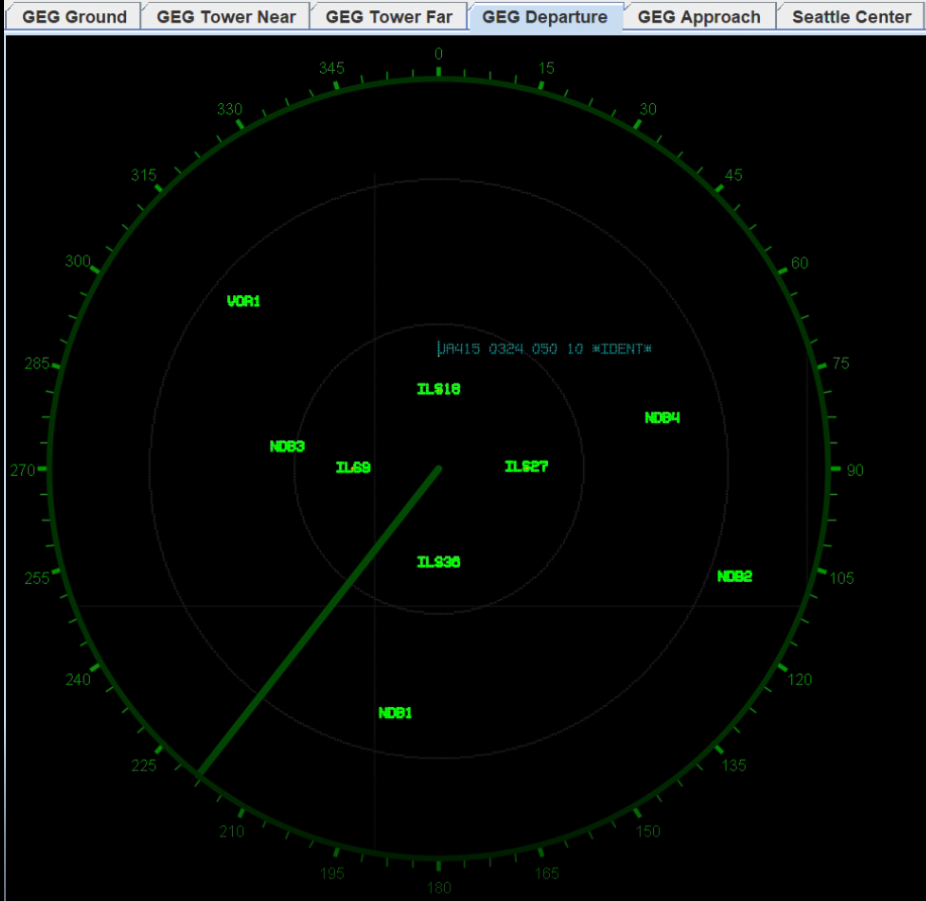
\includegraphics[scale=.4,valign=t]{test1.png}
\item A brief discussion on how the actual results differ from the expected results, if they differ.
\end{enumerate}

\subsection{Test 2: Simple Straight Climb}
Instruct UA415 to climb straight ahead and maintain flight level 240.
\begin{enumerate}
\item The rationale behind the test; i.e., what is it testing and why we care.
\item A general English description of the conditions of the test.
\item The commands for (2), which must appear in a standalone form that could be directly copied into a text file to reproduce
\item the test without manual intervention. Do not cross-reference tests; instead, repeat duplicated code.
\item An English narrative of the expected results of executing the test. Consider this before running the test.
% \item 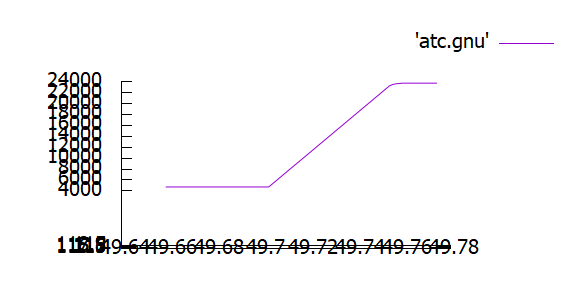
\includegraphics[scale=.4,valign=t]{test2.png}
\item A brief discussion on how the actual results differ from the expected results, if they differ.
\end{enumerate}

\subsection{Test 3: Compound Straight Climb}
Instruct UA415 to climb straight ahead and maintain flight level 320, then upon arriving descend to 15,000 feet.
\begin{enumerate}
\item The rationale behind the test; i.e., what is it testing and why we care.
\item A general English description of the conditions of the test.
\item The commands for (2), which must appear in a standalone form that could be directly copied into a text file to reproduce
\item the test without manual intervention. Do not cross-reference tests; instead, repeat duplicated code.
\item An English narrative of the expected results of executing the test. Consider this before running the test.
% \item 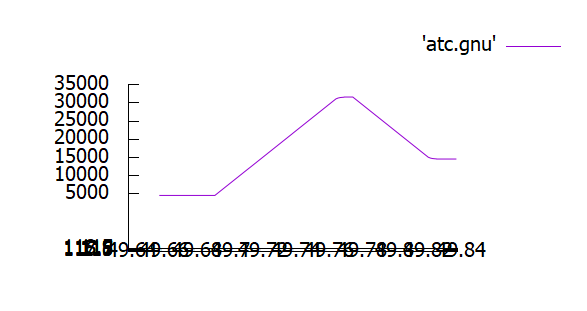
\includegraphics[scale=.4,valign=t]{test3.png}
\item A brief discussion on how the actual results differ from the expected results, if they differ.
\end{enumerate}

\subsection{Test 4: Simple Level Turn}
Instruct UA415 to turn right to 135 degrees.
\begin{enumerate}
\item The rationale behind the test; i.e., what is it testing and why we care.
\item A general English description of the conditions of the test.
\item The commands for (2), which must appear in a standalone form that could be directly copied into a text file to reproduce
\item the test without manual intervention. Do not cross-reference tests; instead, repeat duplicated code.
\item An English narrative of the expected results of executing the test. Consider this before running the test.
% \item \includegraphics[scale=.4,valign=t]{test4.png}
\item A brief discussion on how the actual results differ from the expected results, if they differ.
\end{enumerate}

\subsection{Test 5: Compound Level Turn}
Instruct UA415 to turn left to 270 degrees, then upon arriving right to 090.
\begin{enumerate}
\item The rationale behind the test; i.e., what is it testing and why we care.
\item A general English description of the conditions of the test.
\item The commands for (2), which must appear in a standalone form that could be directly copied into a text file to reproduce
\item the test without manual intervention. Do not cross-reference tests; instead, repeat duplicated code.
\item An English narrative of the expected results of executing the test. Consider this before running the test.
% \item 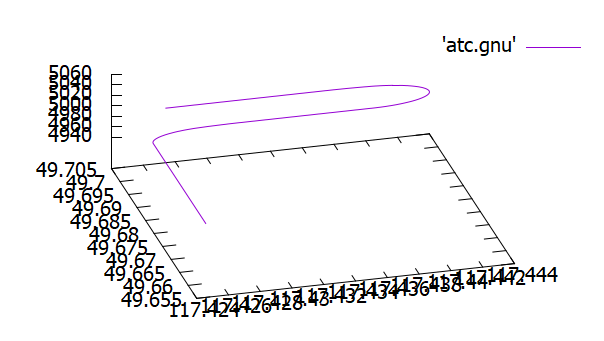
\includegraphics[scale=.4,valign=t]{test5.png}
\item A brief discussion on how the actual results differ from the expected results, if they differ.
\end{enumerate}

\subsection{Test 6: Simple Speed Change}
Instruct UA415 to increase speed to 200 knots (entered as 20).
\begin{enumerate}
\item The rationale behind the test; i.e., what is it testing and why we care.
\item A general English description of the conditions of the test.
\item \begin{verbatim}UA415 increase speed to 20\end{verbatim}
\item the test without manual intervention. Do not cross-reference tests; instead, repeat duplicated code.
\item An English narrative of the expected results of executing the test. Consider this before running the test.
\item 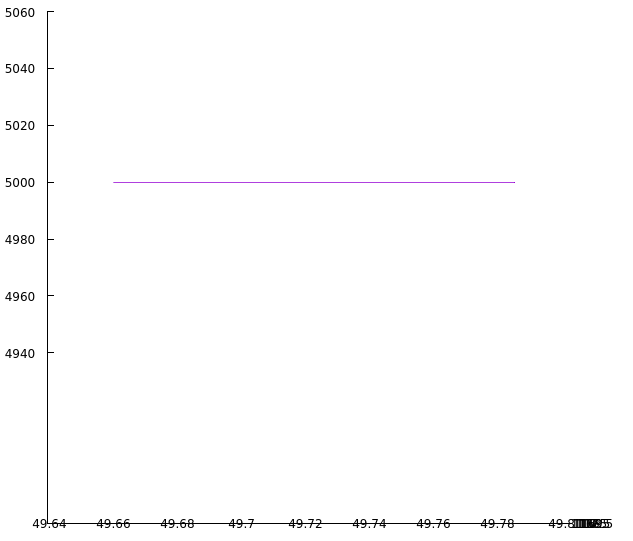
\includegraphics[scale=.4,valign=t]{test6.png}
\item A brief discussion on how the actual results differ from the expected results, if they differ.
\end{enumerate}

\subsection{Test 7: Compound Speed Change}
Instruct UA415 to increase speed to 250 knots, then upon arriving reduce speed to 100.

\begin{enumerate}
\item The rationale behind the test; i.e., what is it testing and why we care.
\item A general English description of the conditions of the test.
\item The commands for (2), which must appear in a standalone form that could be directly copied into a text file to reproduce
\item the test without manual intervention. Do not cross-reference tests; instead, repeat duplicated code.
\item An English narrative of the expected results of executing the test. Consider this before running the test.
% \item 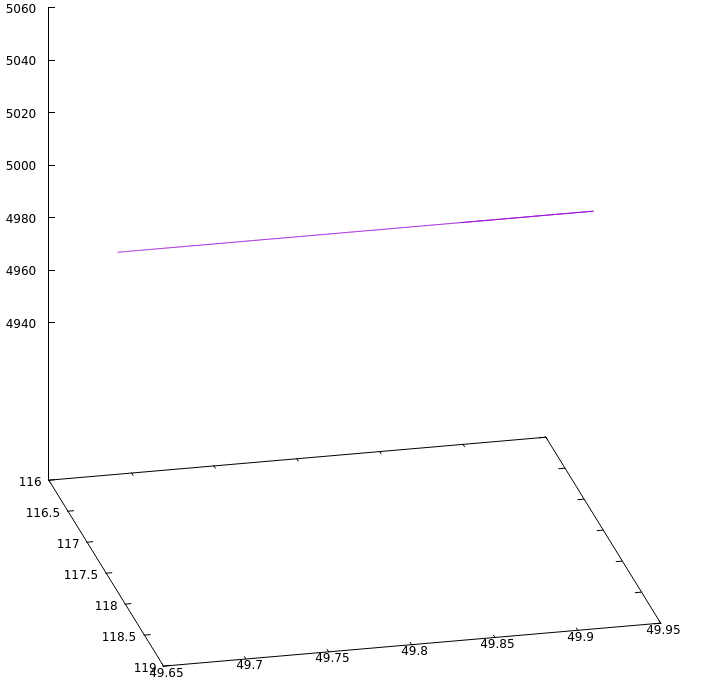
\includegraphics[scale=.4,valign=t]{test7.png}
\item A brief discussion on how the actual results differ from the expected results, if they differ.
\end{enumerate}

\subsection{Test 8: Descending Turn}
Instruct UA415 to climb to flight level 240 to start the test (ignore this setup in the results). Upon arriving, descend to 8,000 feet while turning left to 010.
\begin{enumerate}
\item The rationale behind the test; i.e., what is it testing and why we care.
\item A general English description of the conditions of the test.
\item The commands for (2), which must appear in a standalone form that could be directly copied into a text file to reproduce
\item the test without manual intervention. Do not cross-reference tests; instead, repeat duplicated code.
\item An English narrative of the expected results of executing the test. Consider this before running the test.
% \item 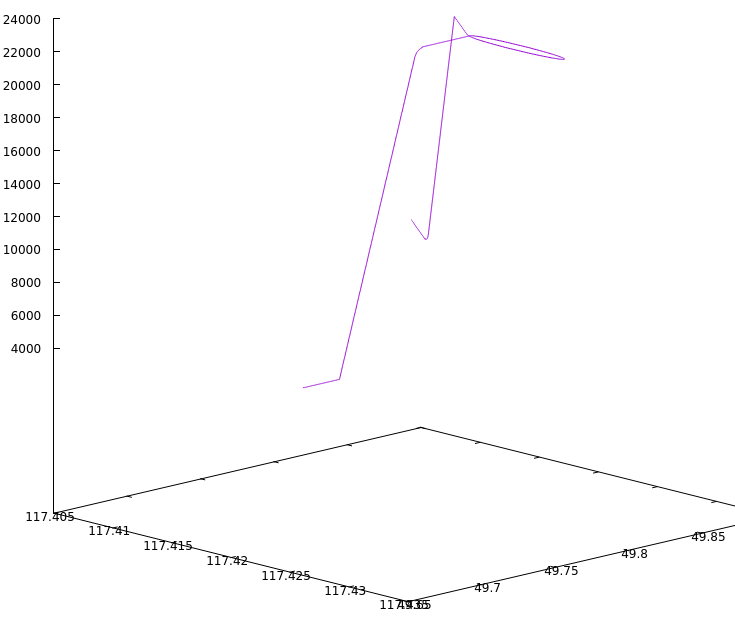
\includegraphics[scale=.4,valign=t]{test8.png}
\item A brief discussion on how the actual results differ from the expected results, if they differ.
\end{enumerate}

\subsection{Test 9: Turn Radius Comparison}
This involves three independent tests with combined results. Use Excel for a top-view plot.
9a. Instruct UA415 to turn right to 270.
9b. Instruct UA415 to turn right to 270 and increase speed to 30.
9c. Instruct UA415 to turn right to 270 and increase speed to 50.
CS 350 Project Specification v0.6 Last Updated 2021-11-30 Page 14 of 15
The following tests demonstrate basic navigation.
\begin{enumerate}
\item The rationale behind the test; i.e., what is it testing and why we care.
\item A general English description of the conditions of the test.
\item The commands for (2), which must appear in a standalone form that could be directly copied into a text file to reproduce
\item the test without manual intervention. Do not cross-reference tests; instead, repeat duplicated code.
\item An English narrative of the expected results of executing the test. Consider this before running the test.
% \item \includegraphics[scale=.4,valign=t]{test9.png}
\item A brief discussion on how the actual results differ from the expected results, if they differ.
\end{enumerate}

\subsection{Test 10: Proceed to Fix, Level}
Instruct UA415 to proceed to fix NDB4.
\begin{enumerate}
\item The rationale behind the test; i.e., what is it testing and why we care.
\item A general English description of the conditions of the test.
\item The commands for (2), which must appear in a standalone form that could be directly copied into a text file to reproduce
\item the test without manual intervention. Do not cross-reference tests; instead, repeat duplicated code.
\item An English narrative of the expected results of executing the test. Consider this before running the test.
% \item \includegraphics[scale=.4,valign=t]{test10.png}
\item A brief discussion on how the actual results differ from the expected results, if they differ.
\end{enumerate}

\subsection{Test 11: Proceed to Fix, Climbing}
Instruct UA415 to proceed to fix NDB4.
\begin{enumerate}
\item The rationale behind the test; i.e., what is it testing and why we care.
\item A general English description of the conditions of the test.
\item The commands for (2), which must appear in a standalone form that could be directly copied into a text file to reproduce
\item the test without manual intervention. Do not cross-reference tests; instead, repeat duplicated code.
\item An English narrative of the expected results of executing the test. Consider this before running the test.
% \item \includegraphics[scale=.4,valign=t]{test11.png}
\item A brief discussion on how the actual results differ from the expected results, if they differ.
\end{enumerate}

\subsection{Test 12: Proceed to Fixes, Altitude Changes}
Instruct UA415 to proceed to fix NDB4 and cross it at flight level 200, NDB2 at 100, NDB1 and 240.
\begin{enumerate}
\item The rationale behind the test; i.e., what is it testing and why we care.
\item A general English description of the conditions of the test.
\item The commands for (2), which must appear in a standalone form that could be directly copied into a text file to reproduce
\item the test without manual intervention. Do not cross-reference tests; instead, repeat duplicated code.
\item An English narrative of the expected results of executing the test. Consider this before running the test.
% \item \includegraphics[scale=.4,valign=t]{test12.png}
\item A brief discussion on how the actual results differ from the expected results, if they differ.
\end{enumerate}

\subsection{Test 13: Proceed to Fix, Climbing and Hold 1}
Instruct UA415 to proceed to fix NDB3 and hold.
\begin{enumerate}
\item The rationale behind the test; i.e., what is it testing and why we care.
\item A general English description of the conditions of the test.
\item The commands for (2), which must appear in a standalone form that could be directly copied into a text file to reproduce
\item the test without manual intervention. Do not cross-reference tests; instead, repeat duplicated code.
\item An English narrative of the expected results of executing the test. Consider this before running the test.
% \item \includegraphics[scale=.4,valign=t]{test13.png}
\item A brief discussion on how the actual results differ from the expected results, if they differ.
\end{enumerate}

\subsection{Test 14: Proceed to Fix, Climbing and Hold 2}
Instruct UA415 to proceed to fix NDB4 and hold.
Explain how Tests 13 and 14 differ.
\begin{enumerate}
\item The rationale behind the test; i.e., what is it testing and why we care.
\item A general English description of the conditions of the test.
\item The commands for (2), which must appear in a standalone form that could be directly copied into a text file to reproduce
\item the test without manual intervention. Do not cross-reference tests; instead, repeat duplicated code.
\item An English narrative of the expected results of executing the test. Consider this before running the test.
% \item \includegraphics[scale=.4,valign=t]{test14.png}
\item A brief discussion on how the actual results differ from the expected results, if they differ.
\end{enumerate}

\subsection{Test 15: Proceed to Fix, Procedure Turn}
Instruct UA415 to proceed to fix NDB4 and execute the procedure turn for runway 22.
\begin{enumerate}
\item The rationale behind the test; i.e., what is it testing and why we care.
\item A general English description of the conditions of the test.
\item The commands for (2), which must appear in a standalone form that could be directly copied into a text file to reproduce
\item the test without manual intervention. Do not cross-reference tests; instead, repeat duplicated code.
\item An English narrative of the expected results of executing the test. Consider this before running the test.
% \item \includegraphics[scale=.4,valign=t]{test15.png}
\item A brief discussion on how the actual results differ from the expected results, if they differ.
\end{enumerate}
\end{document}
